%% 
%% Copyright 2007, 2008, 2009 Elsevier Ltd
%% 
%% This file is part of the 'Elsarticle Bundle'.
%% ---------------------------------------------
%% 
%% It may be distributed under the conditions of the LaTeX Project Public
%% License, either version 1.2 of this license or (at your option) any
%% later version.  The latest version of this license is in
%%    http://www.latex-project.org/lppl.txt
%% and version 1.2 or later is part of all distributions of LaTeX
%% version 1999/12/01 or later.
%% 
%% The list of all files belonging to the 'Elsarticle Bundle' is
%% given in the file `manifest.txt'.
%% 

%% Template article for Elsevier's document class `elsarticle'
%% with numbered style bibliographic references
%% SP 2008/03/01

%\documentclass[preprint,12pt]{elsarticle}

%% Use the option review to obtain double line spacing
%% \documentclass[authoryear,preprint,review,12pt]{elsarticle}

%% Use the options 1p,twocolumn; 3p; 3p,twocolumn; 5p; or 5p,twocolumn
%% for a journal layout:
%% \documentclass[final,1p,times]{elsarticle}
%% \documentclass[final,1p,times,twocolumn]{elsarticle}
%% \documentclass[final,3p,times]{elsarticle}
%% \documentclass[final,3p,times,twocolumn]{elsarticle}
 \documentclass[final,5p,times]{elsarticle}
%% \documentclass[final,5p,times,twocolumn]{elsarticle}

%% For including figures, graphicx.sty has been loaded in
%% elsarticle.cls. If you prefer to use the old commands
%% please give \usepackage{epsfig}

%% The amssymb package provides various useful mathematical symbols
\usepackage{amssymb}
%% The amsthm package provides extended theorem environments
%% \usepackage{amsthm}

%% The lineno packages adds line numbers. Start line numbering with
%% \begin{linenumbers}, end it with \end{linenumbers}. Or switch it on
%% for the whole article with \linenumbers.
%% \usepackage{lineno}

\usepackage{algorithm}
\usepackage{algorithmic}

\journal{Parallel Computing}

\begin{document}

\begin{frontmatter}

%% Title, authors and addresses

%% use the tnoteref command within \title for footnotes;
%% use the tnotetext command for theassociated footnote;
%% use the fnref command within \author or \address for footnotes;
%% use the fntext command for theassociated footnote;
%% use the corref command within \author for corresponding author footnotes;
%% use the cortext command for theassociated footnote;
%% use the ead command for the email address,
%% and the form \ead[url] for the home page:
%% \title{Title\tnoteref{label1}}
%% \tnotetext[label1]{}
%% \author{Name\corref{cor1}\fnref{label2}}
%% \ead{email address}
%% \ead[url]{home page}
%% \fntext[label2]{}
%% \cortext[cor1]{}
%% \address{Address\fnref{label3}}
%% \fntext[label3]{}

\title{Improving Data Movement Performance for Sparse Data Patterns on the Blue Gene/Q Supercomputer}

%% use optional labels to link authors explicitly to addresses:
%% \author[label1,label2]{}
%% \address[label1]{}
%% \address[label2]{}

\author[evl]{Huy Bui}
\author[mcs]{Eun-Sung Jung}
\author[mcs]{Venkatram Vishwanath}
\author[evl]{Andrew Johnson}
\author[evl]{Jason Leigh}
\author[alcf,niu]{Michael E. Papka}

\address[evl]{Electronic Visualization Laboratory (EVL), University of Illinois at Chicago, 842 W Taylor St, Chicago, IL 60607, USA}
\address[mcs]{Mathematics and Computer Science, Argonne National Laboratory, 9700 S Cass Ave, Lemont, IL 60439, USA}
\address[alcf]{Argonne Leadership Computing Facility, Argonne National Laboratory, 9700 S Cass Ave, Lemont, IL 60439, IL, USA}
\address[niu]{Northern Illinois University, 300 Normal Road, DeKalb, IL 60115, USA}

\begin{abstract}

In-situ analysis has been proposed as a promising solution to glean faster insight and to reduce the amount of data written out to storage. A critical challenge here is that the reduced dataset needed to visualize a specific region of interest as the simulation is running is typically held on a subset of the nodes and needs to be written out to storage. Coupled multiphysics simulations also produce a sparse data pattern wherein data movement occurs among a subset of nodes. We evaluate the performance of these data patterns and propose several mechanisms for improving performance. Our mechanisms introduce intermediate nodes to implement multiple paths to transfer data on top of default routing algorithms and utilize topology-aware data aggregation to avoid shared bottleneck links. The efficacy of our solutions is evaluated through microbenchmarks and application benchmarks on an IBM Blue Gene/Q system scaling up to 131,072 compute cores. The results show that our algorithms achieve up to a 2X improvement in achievable throughput compared to the default mechanisms.

\end{abstract}

\begin{keyword}
multiple paths \sep sparse data movement \sep topology-aware aggregation \sep data-intensive \sep Blue Gene/Q
%% keywords here, in the form: keyword \sep keyword

%% PACS codes here, in the form: \PACS code \sep code

%% MSC codes here, in the form: \MSC code \sep code
%% or \MSC[2008] code \sep code (2000 is the default)

\end{keyword}

\end{frontmatter}

%% \linenumbers

\section{Introduction}
\label{sec:intro}
Simulation time in a supercomputer depends partially in achievable networking performance in the supercomputer. The achievable networking performance in its turn depends on the exact combination of communication patterns of applications and routing algorithms used by the supercomputer. For each communication pattern there exists routing algorithms resulting in optimal networking performance. However, while the communication patterns have wide spectrum and vary time to time, the routing algorithms have a limited variation and usually are optimized for typical communication patters. This results in high networking performance for favored communication patterns but low networking performance for other communication patterns. Low networking performance subsequentially leads to long simulation time. Reducing the communication time for these non-favored communication patterns reduces the running time of the applications. Thus, improving the networking performance for these communication patterns are important in redecing simulation time. 

The low performance in non-favored communication patterns are due to the unblanced on physically links caused by changing in the communication patterns. Rebalancing loads on the physical links in these situations can lead to better achievable performance. 

In this work, we focus on group communication, in which a set of M source nodes communicates with a set of N destination nodes. The M nodes can be disjoint from the set of N nodes as appearing in many applications. The can also be overlap such as in The Model Coupling Toolkit (MCT) of Community Earth System Model (CESM) applications \cite{MCT:Jacob}, or can be subset such as in I/O aggregation \cite{Vishwanath:GLEAN}. The pairing between nodes in the two sets can be aligned or can be randomly depending on the applications' patterns.

We propose two approaches that improve network performance for applications in supercomputers by rebalancing the load on physical links. Our approaches include a heuristic algorithm and a formal model with mathematical solvers to search for paths to move data from a set of sources to a set of destinations. The data then is divided into smaller messages and put into queues to move along found paths. The actual data movement can be done by using any available libraries for communication on the supercompter. We realize our approaches in a framework called OPTIQ. Our framework allows to easily expand our work by adding algorithms for search paths, different ways to schedule data transfer and different ways to transfer data. It also allows to extend the framwork to other systems.

Our contributions include:
\begin{itemize}
\item Bring an insight understanding of how networking happens in the Blue Gene/Q supercomputer. By experiments, we show patterns that current routing algorithms favor and what it doesn not and explain why it happens it that way.
\item Propose a set of approaches to improve networking throughput by taking advantage of unused links or balancing network on links.
\end{itemize}

Our paper includes the follows. In the next section, we present previous works in improving and optimizing data movement in various supercomputers or computing systems. We then give a brief introduction of our framework OPTIQ in \ref{sec:framework}. The details of our approaches are presented in section \ref{sec:approach}. We demonstrate the efficacy of our approaches via a set of benchmarks in section \ref{sec:benchmark}. In section \ref{sec:conclusion}, we conclude our work and give some ideas about future work.


\section{Related work}
\label{sec:relatedwork}

GOAL paper \cite{singh2003:goal}
Several bgq paper

In our previous works in \cite{Vishwanath:GLEAN}, \cite{SDAV:Bui2014b}, \cite{hbui:bgq} we have already presented our approaches for improving the performance of data movement for certain cases very dense in I/O case, or very sparse in p2s2. In this paper, we give solution for medium dense communication patterns between M and N.


\subsection{Experiment system}
\label{sec:system}

Mira \cite{Chen:BGQ}, with 48 compute racks (48K nodes and 768K cores) at the ALCF, provides 10 PFlops theoretical peak performance. Each node has a 16-core processor and 16 GB of memory.

The interprocess communications of Blue Gene/Q travel on a 5D torus network both for point-to-point and for collective communications. This 5D torus interconnects a compute node with its 10 neighbors at 2 GB/s theoretical peak over each link in each direction, making a total of 40 GB/s bandwidth in both directions for a single compute node. Because of packet and protocol overheads, however, only up to 90\% of the raw data rate (1.8 GB/s) is available for user data. The machine can be partitioned into non-overlapping rectangular submachines; these submachines do not interfere with each other except for I/O nodes and the corresponding storage system.

For interconnect network traffic, BG/Q supports both deterministic and dynamic routing \cite{Chen:BGQ}. In the dynamic routing, messages in different message size ranges can be routed differently. However, within a given message size range, routing is always the same, and its path is known before it is routed. These are the default routing algorithms and cannot be changed during run time. The BG/Q supercomputer uses single-path data routing, for sending/receiving a message only one link of the ten available is used. The details of routing can be found in \cite{Chen:BGQ}.

PAMI is a low-level communication library for BG/Q \cite{PAMI:Kumar}. PAMI provides low-overhead communication by using various techniques such as accelerating communication using threads, scalable atomic primitives, and lockless algorithms to increase the messaging rate. Since MPI is implemented on top of PAMI, direct use of PAMI would provide higher messaging rates as well as lower latencies in comparison with MPI.




\section{Approaches}
\label{sec:approach}

In the Blue Gene Q supercomputers, data transfers are routed using default routing algorithm. The default routing algorithm is proved to be well-balanced in many communication patterns \cite{Chen:BGQ}. However, for certain communication patterns, it results in poor performance due to unbalanced networking load on physical links, in which some links serve more amount of data transferred through than other links. Those links become bottleneck in data movement. In order to improve performance, we propose four approaches aiming for balancing load on physical links. We also give a brief description of a framework called OPTIQ, a realization of our approaches.

\subsection{Path searching approaches}
Our approaches aim to balance networking load among physical links. To do so, we first model the interconnect network as a graph, in which each compute node is modeled as a vertex and each physical link is modeled as an edge. The bandwidth of a physical link is modeled as its corresponding edge's capacity. The need of data movement from source nodes to destination nodes is modeled as data movement from source vertices to destination vertices. After we construct the graph, we search for paths to transfer data from source vertices to destination vertices. We apply constraints when searching for paths to balance number of paths that use a certain link. Each pair of source-destination may have more than one path to transfer data. Thus, we need to split the data among those paths to balance the actual amount of data transferred through physical links.

Four approaches that we present in this section include two heuristic algorithms, one multiple paths data movement taking advantages of existing shortest paths algorithms and one model-based approach. All paths searching algorihtms here are centric algorithms. They run at every node in exact order. Hence, every node has the same results. We build the graph with system's information such as size, topology, torus of the partition, coordinates of all nodes in the partition. The information is collected once at the begining. The inputs of the algorithms are source and destination vertices and amount of data to be transferred from the sources to the destinations. We present in detail each approach below.

\subsubsection{Heuristic 1 - Breadth first search based}

In this approach, we search for paths between each pair of source and destination. From a source, we explore from all the destination in all possible directions. Whenever we reach a destination, we mark the destination as found to no longer search for it on other explorering paths from the same source. In this algorithm, we limit exploring paths by constraints of number of hops and maximum load. The algorithm is described in \textbf{Algorithm \ref{alg:h1}}.

\begin{algorithm}[!htp]
\textbf{Input:} Set of pairs of source-destination (\textit{s$_i$, d$_i$}). Number of nodes \textit{n}. Graph of nodes. \\
\textbf{Output:} Set of paths: one path for a pair of source-destination \\
\\
Structures:
\begin{algorithmic}
\State struct arc \{int u, int v\};
\State struct path \{set of arcs\};
\end{algorithmic}

Heap element comparison:
    \begin{algorithmic}
	\Function{heap\_compare} {path p1, path p2, int maxload, int maxhops}
	    \If {both paths has max load greater than maxload} 
		\State choose the one with smaller number of hops.
	    \EndIf
	    \If {One path has max load greater but one path has max load smaller than maxload}
		\State Choose the one with smaller load.
	    \EndIf
        \EndFunction
    \end{algorithmic}

Init:
    \begin{algorithmic}
	\State min\_heap$<$struct path$>$ \textit{exploring\_paths} = $\varnothing$;
	\State queue$<$struct path$>$ \textit{complete\_paths} = $\varnothing$;
	\State bool \textit{visisted}[\textit{n}][\textit{n}];
	\For {0 $<=$ {\it i}, \textit{j} $<$ \textit{n}} 
	    \State \textit{visited}[{\it i}][{\it j}] = false;
	\EndFor
    \end{algorithmic}
Main:

\begin{algorithmic}
    \Function {Heuristic\_search\_I}{}

    \While {exist a source \textit{s$_i$} with unvisted neighbor \textit{u}}
	\State check\_and\_add\_new\_path({\it s}$_i$, \textit{u}, null);
	\State Pick next \textit{s$_i$} in the sources
    \EndWhile

    \While {(\textit{exploring\_paths} != $\varnothing$)}
	\State path \textit{p} = \textit{exploring\_paths}.extract\_min();
	\State {\it u} = last vertex in the path {\it p};
	\For {each neighbor \textit{v} of \textit{u}}
	    \State check\_and\_add\_new\_path({\it u}, \textit{v}, {\it p});
	\EndFor
    \EndWhile

    \EndFunction
\\
    \Function{check\_and\_add\_new\_path}{int \textit{u}, int \textit{v}, path {\it op}}
	\If {(!{\it visited}[{\it u}][{\it v}])}
	    \State create a path \textit{np} = {\it op}
	    \State add arc $<$\textit{u}, \textit{v}$>$ to \textit{np}
	    \State enqueue \textit{np} to \textit{exploring\_paths}
	    \If {{\it v} is one of the destinations of \textit{s$_i$} of \textit{np}}
	        \State enqueue \textit{np} to \textit{complete\_paths}
            \EndIf
	    \State {\it visited}[\textit{u}][\textit{v}] = true;
	\EndIf
    \EndFunction
\end{algorithmic}

\caption{Heuristic Alg 1: Exploring all paths without constraints}
\label{alg:h1}

\end{algorithm}

The \textbf{Algorithm \ref{alg:h1}} can be divided into 2 parts. In the first part, which is in the first \textbf{while} loop of the function Heuristic\_search\_I, we start at every source and add 1-hop paths to \textit{exploring\_paths} queue. Those paths are the paths from sources to their neighbors. We need a \textit{break} statement after each adding to make sure that every source can a path before they can all start again. This is to help ...

In the second part, which is the second \textbf{while} loop of the function Heuristic\_search\_I, we pop an exploring path \textit{p}from the \textit{exploring\_paths}. From the last added vertex \textit{u} of \textit{p}, we exploring all edges from it to it neighbors and add new path \textit{np} = \textit{p} + newly explored edge. If any of its neighbors is final destination of source \textit{s$_i$}, we then add \textit{np} into \textit{complete\_paths}. We continue the work until all the paths are explored.

Time complexity: The graph has V vertices and E edges. We have K pairs of (source, destinatinon), each source has at most D neighborhoods, then the time complexity of the \textbf{Algorithm \ref{alg:h1}} is $O$(K * ($|$V$|$ + $|$E$|$)). The time complexity is breakdown as following:
\begin{itemize}
\item First part: we have K pairs hence K sources, for each source we discover its D neighbors, thus time will be $O$(K*D).
\item Second part: For this part, we get a path out of \textit{exploring\_paths}, create new paths by exploring its neighbors that are not visited by its source and add the new paths back to \textit{exploring\_paths}. For each sources, every vertex and every edge can be visited in the worst case, the time complexity would be $O$($|$V$|$ + $|$E$|$) minus to the vertices and edges visited by the first part. As we have K sources, the time complexity is $O$(K * ($|$V$|$ + $|$E$|$)).
\end{itemize}

\subsubsection{Heuristic 2 - Path-based approach}

\begin{algorithm}[!htp]
\textbf{Input:} Set of pairs of source-destination (\textit{s$_i$, d$_i$}). Number of nodes \textit{n}. Graph of nodes. Number of shortest path \textit{k}\\
\textbf{Output:} Set of paths: \textit{k} paths for a pair of source-destination\\
Init:
    \begin{algorithmic}
        \State queue$<$struct path$>$ \textit{complete\_paths};
    \end{algorithmic}
Main:
\begin{algorithmic}
    \Function {Heuristic\_search\_II}{}
	\For {each pair of source-dest (\textit{s$_i$}, \textit{s$_i$})}
	    \While{less than k paths discovered || still have paths to discover}
		\State Use Yen's algorithm to search for the shortest path \textit{p}.
		\State Check if adding \textit{p} make the current load over max load.
		\State If not, add \textit{p} into \textit{complete\_paths}
	    \EndWhile
	\EndFor
    \EndFunction
\end{algorithmic}

\caption{Heuristic Alg 2: k shortest paths}
\label{alg:h2}

\end{algorithm}

In the \textbf{Algorithm \ref{alg:h3}}, we use Yen's algorithm to search for k shortest paths between \textit{s$_i$, d$_i$}.

In Agorithm 1 and 2, we aim on balancing the number of paths using physical link. However, we do not consider the actual amount of data transferred on each path. If multiple paths are found, the data is equally split among the paths. To gain better performance, we determine the amount of data to be transferred on each path by using a mathematical model to search for the amount of data to be transferred on each path. The approach takes a number of given paths and amount of data between 2 vertices and use solvers to search for the amount of data on each path. The detail is described as follows.

\subsubsection{Path-based model optimization}

How do we come up with the model?

Here is the model with its description below.

\begingroup
\fontsize{9pt}{10pt}\selectfont

\begin{verbatim}

set Nodes;
set Arcs within Nodes cross Nodes;

set Jobs;
set Paths{Jobs};
set Path_Arcs{job in Jobs, p in Paths[job]} 
    within Arcs;

param Capacity{Arcs} >= 0 default Infinity;
param Demand {Jobs} default 0;

var Flow {job in Jobs, Paths[job]} >= 0;
var Z >= 0;

maximize obj: Z;

subject to

demand {job in Jobs}:
  sum {p in Paths[job]} Flow[job,p] = Demand[job]*Z;

capacity {(i,j) in Arcs}:
  sum {job in Jobs, p in Paths[job]: (i,j) in 
    Path_Arcs[job,p]} Flow[job,p] <= Capacity[i,j];

\end{verbatim}

\endgroup

Model explanation:
\begin{itemize}
\item sets: we have 5 sets: \textit{Nodes}, \textit{Arcs}, \textit{OD}, \textit{Paths} and \textit{Path\_Arcs}. \textit{JobID}: is the set of transfers from sources to destinations. Each job is represented by a tuple (id, source, destination, demand (total data size to transfer)).
\item params: {\it Capacity}: capacity of each arc; {\it Demand}: amount of data to be transferred in each job between a pair of orgin and destination.
\item vars: \textit{Flow}: total flow of each job on each arc; \textit{Z}: is reversed of total time; \textit{total\_flow} total flow of all jobs going through an arc.
\item objective function: we want to minimize the time or maximize its reversed value i.e. maximize \textit{Z}.
\item constraints(subject to): \textit{zero\_flow}: total flow through a source is total going out of that source, total flow going through a destination is total flow going in that destination, for other nodes that total is 0; \textit{capacity}: total flow on an arc is less than its capacity.
\end{itemize}

We feed the model to solvers and get the paths with given proportional bandwidth. Based on that, we can decide how much data we can transfer alogn each path.

So far, we have presented different algorithms/approaches. Each has its own use case scenario. The Table \ref{tbl:approaches} describes the situation when to use each of them. 

\begin{table}[h]

\begin{center}
    \begin{tabular}{ | p{1cm} | p{2cm} | p{2cm} | p{2cm} |}
    \hline
     & BFS-based &  \multicolumn{2}{ c| }{Path-based} \\ \hline
     & Heuristics 1 & Heuristics 2 & Optimization Model \\ \hline
    Time Complexity & $O$(K * ($|$V$|$ + $|$E$|$)) & $O$(K * (Time complexity of the algrithms used to get k shortest paths)) & $O$(K * (Time complexity of the algrithms used to get k shortest paths) + Solving time) \\ \hline
    When to use & Very dense communication & Sparse comminication &  Medium dense where proportional throughtput can be gained \\
    \hline
    \end{tabular}

    \caption{Approaches: time complexity and usage}
    \label{tbl:approaches}

\end{center}
\end{table}

We realize algoirthms and other work in a framework named OPTIQ. 

\subsection{Framework}

Our framework has 3 main components: Path searching algorithms, Schedule and Transport and an extra component depicted in Figure \ref{fig:framework}.

\begin{figure}[!htb]
\vspace{-0.1in}
\centering
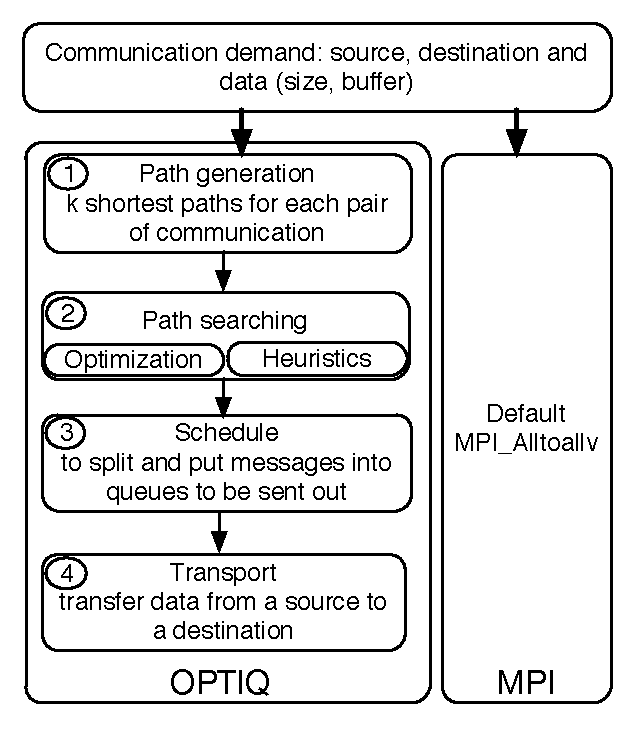
\includegraphics[scale=0.7]{figures/framework.pdf}
\vspace{-0.2in}
\caption{Three components of OPTIQ framework}
\vspace{-0.1in}
\label{fig:framework}
\end{figure}

The functionarity of each component is as following:
\begin{itemize}
\item Path searching: search for path to transfer data from a set of sources to a set of destination. Multiple or single paths can be found using a set of algorithm. User can decide what algorithm to be used or let the framework use a default algorithm.
\item Schedule: Split a buffer data that needed to tranfer into smaller messages and put those messages into a queue of transport layer to be transferred. It also handles incoming messages for itself and for forwardig them to its neighbors on a way to a message final destination.
As we route data in our own ways, we search for the paths, and we also need to schedule messages transfer. It includes sending local messages, forwarding messages form other sources, receiving data as the intermediate node or the destination node.

Order of messages into sending queue: 3 types of messages: local messages (needed to send), fowarding messages (needed to send), its receiving messages. first come first serve, local messages first. forwa

When there are multiple ranks per node, which one will be choosen to receive data at the next dest (forwarding). Single rank to do or many rank to do, currently every rank executes data transfer.

\item Transport: actually transfer an amount of data from one point to another point in the system.
\item Extra component: To get system specific information such as partition size, topology, coordinates, torus, and to compute neighbors of available nodes given to an application. Topology reading, coord, neighbors, torus, size, routing order, graph generated. Also set of benchmarks, tests.

The framework has various options to allow users to tune the framework for optimal performance. For example, the framework allows to select messages from queue to either forward a message from another node first or to send its own message first, to select algorith to search for paths or to set chunk size to transfer a message, to easily add new transport layers on different machine.

\end{itemize}


\section{Microbenchmarks}
\label{sec:microbenchmarks}
In this section, we show the efficacy of our solutions through a set of microbenchmarks for 2 cases: data movement for data coupling nodes and data movement between compute nodes and I/O.

\subsection{Efficacy of proxies and pipeline technique}

%On BG/Q, we tested the system with 16 cores per node all communicate with 16 cores on another node, they transferred in all same links, resulting in 1.7GB/s at most. Due to the symmetry of mapping, it's more likely to all cores belonging to a nodes to connect with all cores belonging another nodes than connect with cores at different nodes. With 20 links per nodes, using multiple paths for data movement on BG/Q can results in significant throughput improvement. 

In this microbenchmark, we transfer data between two nodes through an intermediate nodes using pipelining and compare results with transferring data without using pipeline and with a direct transfer (default) scheme. We varied the data size from 1K  to 128MB.

\begin{figure}[!htb]
\centering
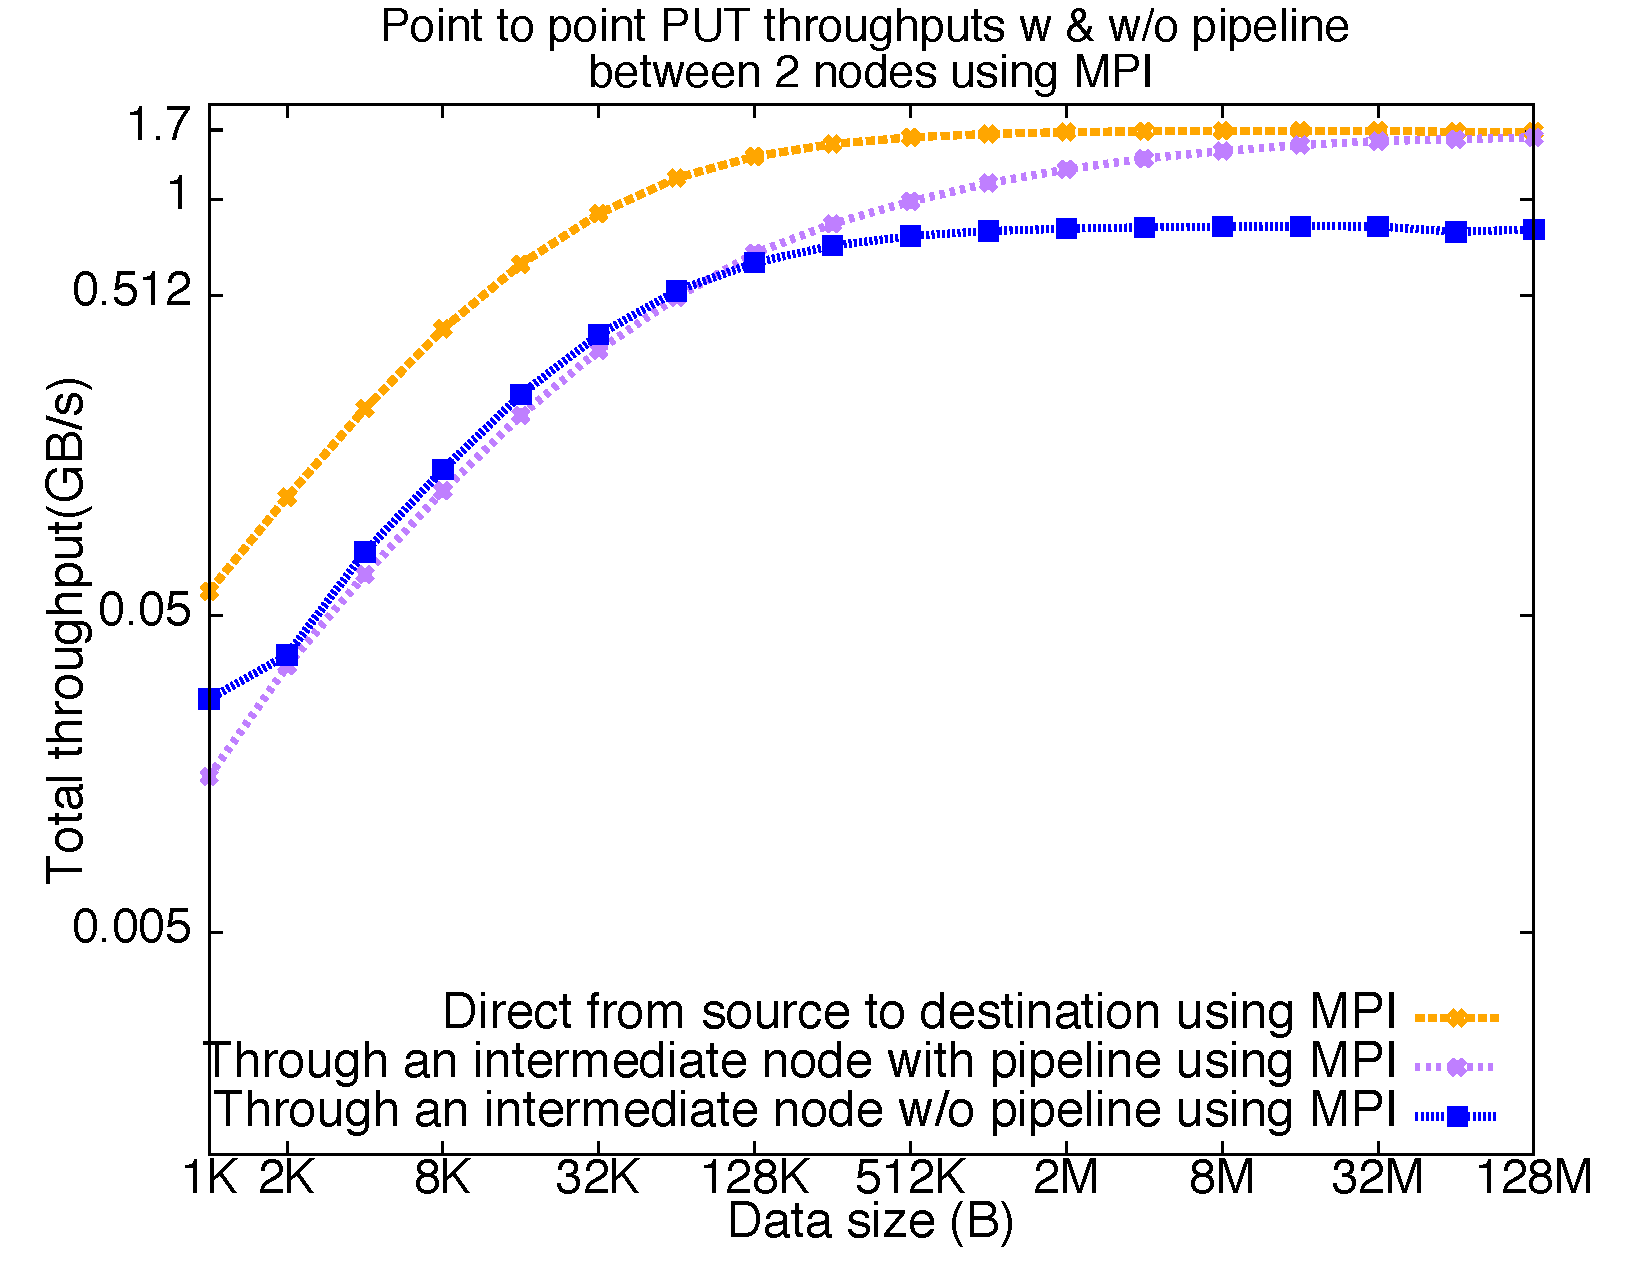
\includegraphics[scale=0.3]{figures/pipeline_mpi.pdf}
\caption{Using pipelining technique to mitigate the waiting time at proxy nodes}
\label{fig:pipeline_mpi}
\end{figure}

Fig. \ref{fig:pipeline_mpi} shows that transferring data through a proxy without using pipelining results a 50\% hit in performance over a direct transfer. This is because the proxy needs to wait until entire data is ready before forwarding it to the destination. By using pipelining, for message less than 64KB,  pipelining does not improve performance, however, for a message size larger than 64KB, pipelining demonstrates an improve performance. At a  message size of 1MB, 2MB, and 4MB, we achieve 70\%, 80\%, and  90\% respectively of the direct transfer bandwidth, and with larger size messages, we achieved a similar performance. Thus, with large size messages, pipelining technique can be used to transfer data through proxies. However, with small size messages, the performance gained is insignificant. Much of the performance overhead is due to the underlying rendezvous protocol design in MPI on the BG/Q. Next, we use PAMI to improve the performance for small messages. The next subsection, we show the efficacy of using PAMI on transferring small size messages.

\subsection{Quantifying computation used for data movement at proxies}
In this section, we quantify the time spent by the CPU for data movement, and we show that it is so small that it has no effect on the total time.

\subsection{Data movement for data coupling nodes}
In this benchmark, we show feasibility of the approach using proxies to increase transfer throughput between 2 compute nodes. We choose the first and the last node of a partition of 128 compute nodes with 2x2x4x4x2 torus. As the partition is large enough we are able to choose 4 proxies to transfer data in 4 directions +B, +C, +D, +E . In each node, only one MPI rank is used (when we use multiple MPI ranks per node to send data to the same destination, they all take the same output link, thus using one MPI rank is still valid and making the experiment easier). The data is transferred in increasing size from 1KB up to 128MB of data, with the size doubled each time. We use MPI\_Put to transfer data from source node to proxy nodes and then from proxy nodes to destination node. Each transfer is repeated multiple times with different data to eliminate any cache effect and achieve stable performance. The average transfer throughput between 2 nodes is reported in Figure \ref{fig:4proxies}.

\begin{figure}[!htb]
\vspace{-0.1in}
\centering
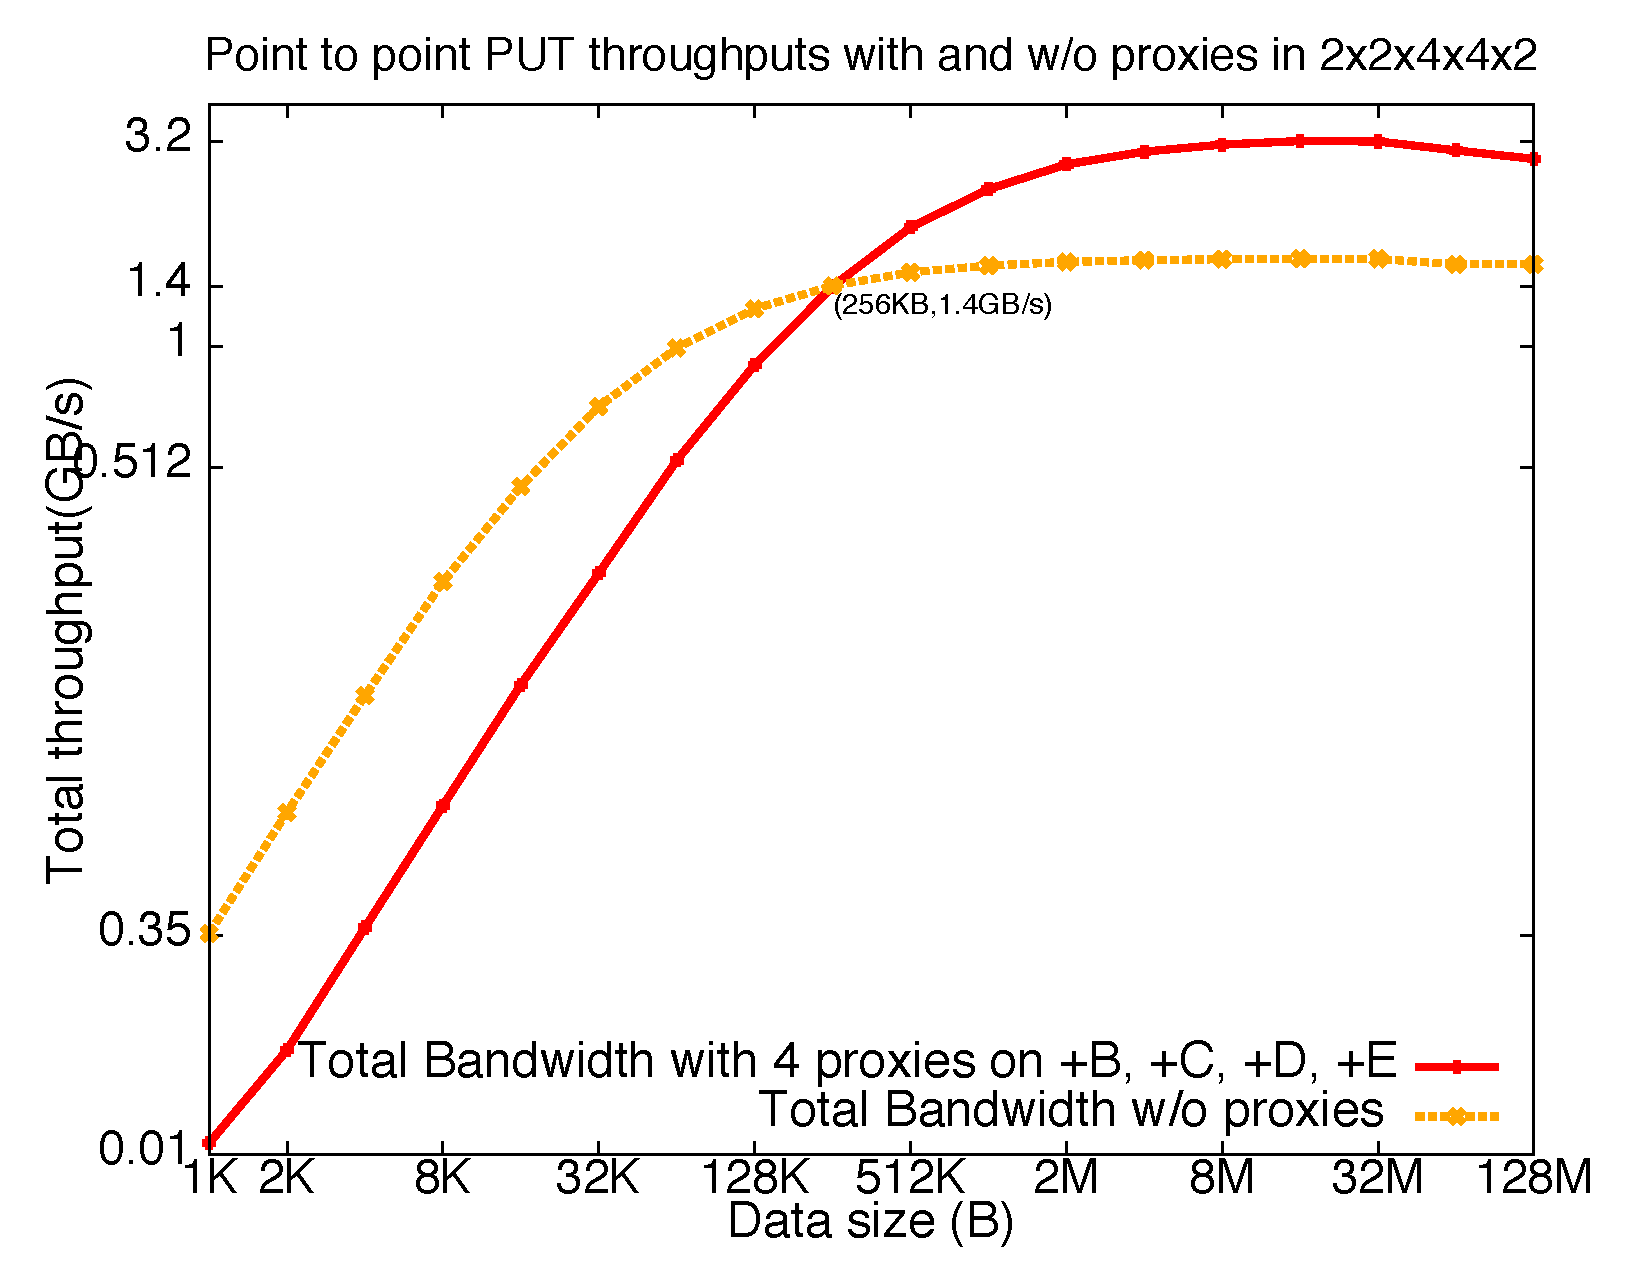
\includegraphics[scale=0.3]{figures/4proxies}
\vspace{-0.2in}
\caption{Using 4 proxies to improve data transfer throughput between 2 nodes}
\vspace{-0.1in}
\label{fig:4proxies}
\end{figure}

As the figure shows, for the small messages, direct transfer yields better performance. With large message, proxy-based transfers outruns direct transfer with $2\times$ better performance. This is foreseen with the reasons we mentioned before: with small messages, extra time caused by injecting and copying messages is significantly larger than the transferring time. It happens in the opposite way with large messages. The message size threshold to switch from direction transfer to proxy-based transfer is 256KB, yielding 1.4GB/s per link. After the threshold, direct transfer slowly reaches to maximum ~1.6BG/s while proxy-based transfer continue to thrive until ~3.2GB/s. Thus, the benchmark shows that proxy-based approach is feasible and can result significant improvement.

As data movement in multiphysics applications is done by more than 2 single nodes, the second benchmark elucidates the feasibility and achievable throughput for data movement between two groups of nodes. In this experiment, we transfer data between two groups of nodes, wherein each group has 256 nodes in a 4x4x4x16x2 torus of a 2K nodes partition. One group is at one corner of the partition, the other one is at the other end of the partition. The data size is also from 1KB to 128MB with doubled size each step. The experiment is repeated for a number of times. We are able to choose 3 proxies for each node. The Figure \ref{fig:3groxies} shows the average throughput measured.

\begin{figure}[!htb]
\vspace{-0.1in}
\centering
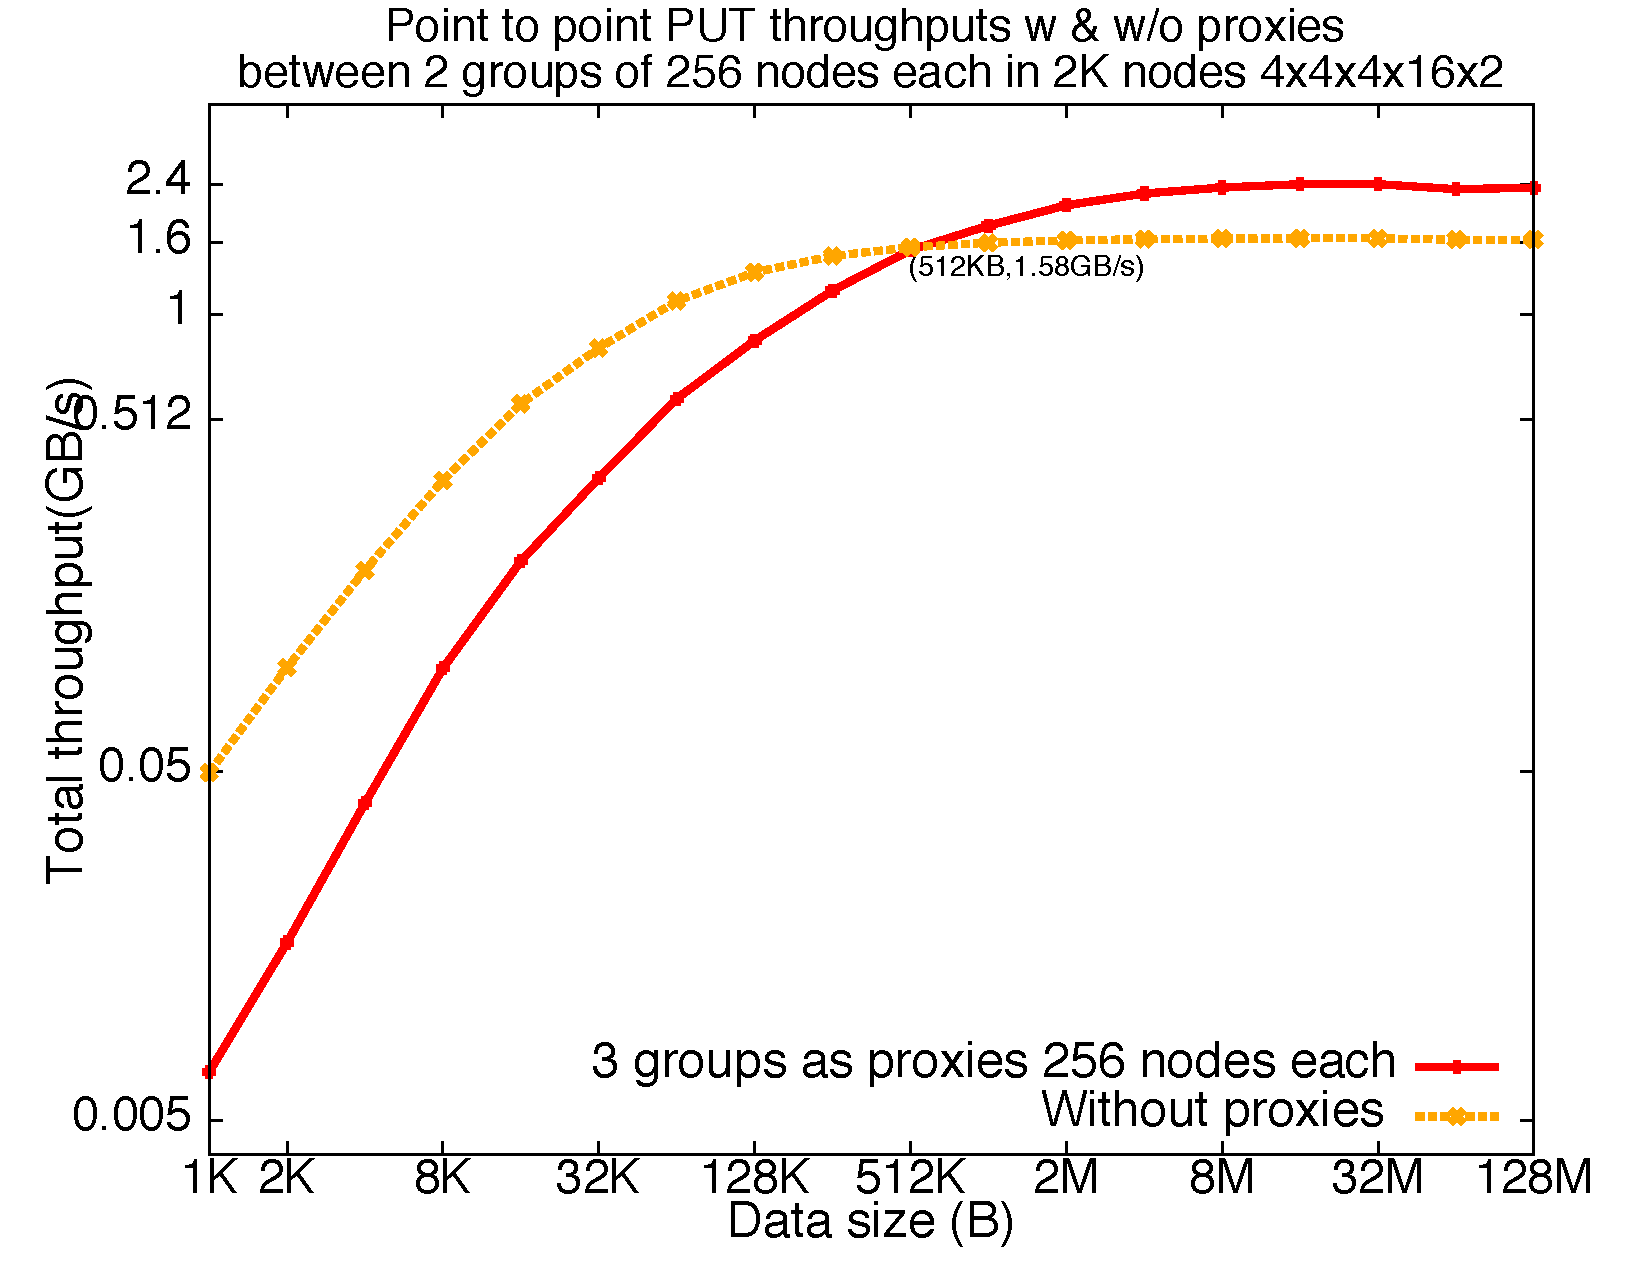
\includegraphics[scale=0.3]{figures/3groxies}
\vspace{-0.2in}
\caption{Using 3 group of proxies to improve data transfer bandwidth between 2 group of nodes}
\vspace{-0.1in}
\label{fig:3groxies}
\end{figure}

In the figure, we once again see that with small messages, direct transfer is better than proxy-based transfer. The threshold for this case increases to 512KB. At that message size, direct transfer also reaches to its maximum throughput, while the proxy-based transfer still has big room to increase up to 2.4GB/s. The performance increases $1.5\times$ as predicted since 3 proxies are used for each nodes. This benchmark shows that proxy-based data transfer is feasible for data transfer between groups of nodes. And we can achieve significant improvement in certain cases.

As we have mentioned in Section \ref{sec:approaches}, we need at least k $>$ 2 proxies per each data transfer to benefit from proxies. The more proxies we can use the better performance we can gain. However, as the size of communicating groups increases, the number of proxies we can set up decreases. If we add more proxies beyond the maximum possible proxies, data movements by extra proxies intervene existing ones and eventually degrade overall performance. The Figure \ref{fig:num_groxies} demonstrates the situation.

\begin{figure}[!htb]
\vspace{-0.1in}
\centering
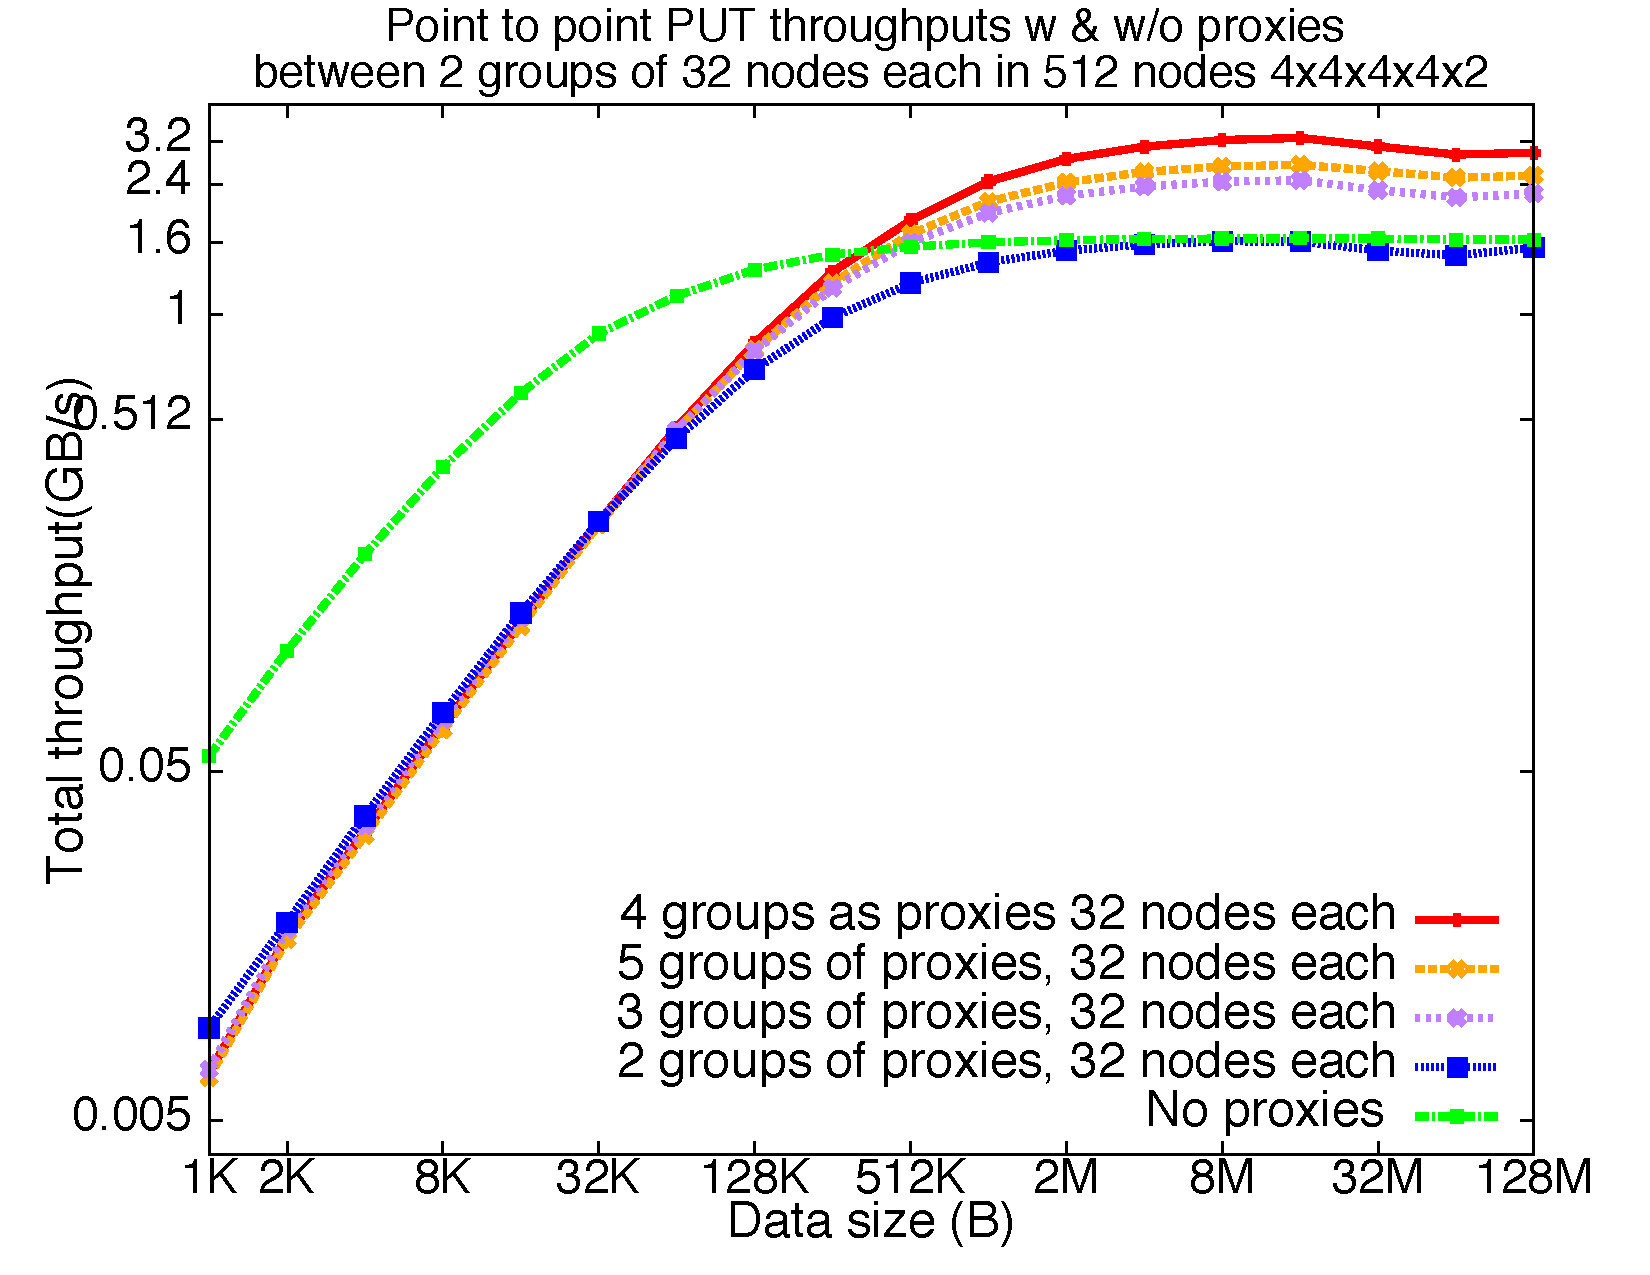
\includegraphics[scale=0.3]{figures/num_groxies}
\vspace{-0.2in}
\caption{Performance variance with number of proxies}
\label{fig:num_groxies}
\vspace{-0.1in}
\end{figure}

With the torus 4x4x4x4x2 and 2 groups of 32 nodes each, we can set up at most 4 groups of proxies along A+, A-, B+, B- dimensions. The 5th proxy is the source node itself. As Figure \ref{fig:num_groxies} shows, when we increases the number groups of proxies from 2 to 3 and to 4, the throughput increases from no-improvement, to 1.5$\times$ and to 2$\times$. Thus, with large message sizes, we can gain k/2 times performance with k being the number of proxies. However, when we increase number of proxies to 5, the performance starts to drop due to intervention among concurrent data movements. Therefore, choosing number of proxies together with their locations is important to maximize throughput.

The above three benchmarks demonstrate the efficaty of our solutions for data movement between compute nodes. In the next subsection, we evaluate our approaches in the case of data movement between compute nodes and I/O nodes. 

%\subsection{Sparse data patterns}


%In the next subsection, we present our benchmarks on the two data patterns generated.
%\subsection{Staging}

\subsection{Data Movement to I/O nodes}
We perform a weak scaling study with two sparse data patterns, and scale the number of cores from 2,048 to 131,072 cores on the Mira BG/Q system. 

\begin{itemize}
\item Pattern 1: Uniform distribution data where data size of a MPI rank is uniformly distributed between 0 and 8MB.  Data is generated by using \textit{srand()} and \textit{rand()} functions in C/C++ and using \textit{time(NULL)} as a seed.  Total data size is about 50\% of the dense data. The distribution of the data size is shown in Figure \ref{fig:uniform}.
\item Pattern 2: Pareto distribution data where many of MPI ranks have data size of 0 bytes or very low size, and a few of MPI ranks have data size of 8MB or close by. The total data size is about 20\% of the dense pattern. The distribution of the data is shown in Figure \ref{fig:pareto}
\end{itemize}

In the data pattern 1, data sizes are uniformly distributed among nodes. This data pattern can be seen when we want to analyze data from different regions with different resolutions. Depending on the resolution, data sizes may vary accordingly.

\begin{figure}[!htb]
\vspace{-0.2in}
\centering
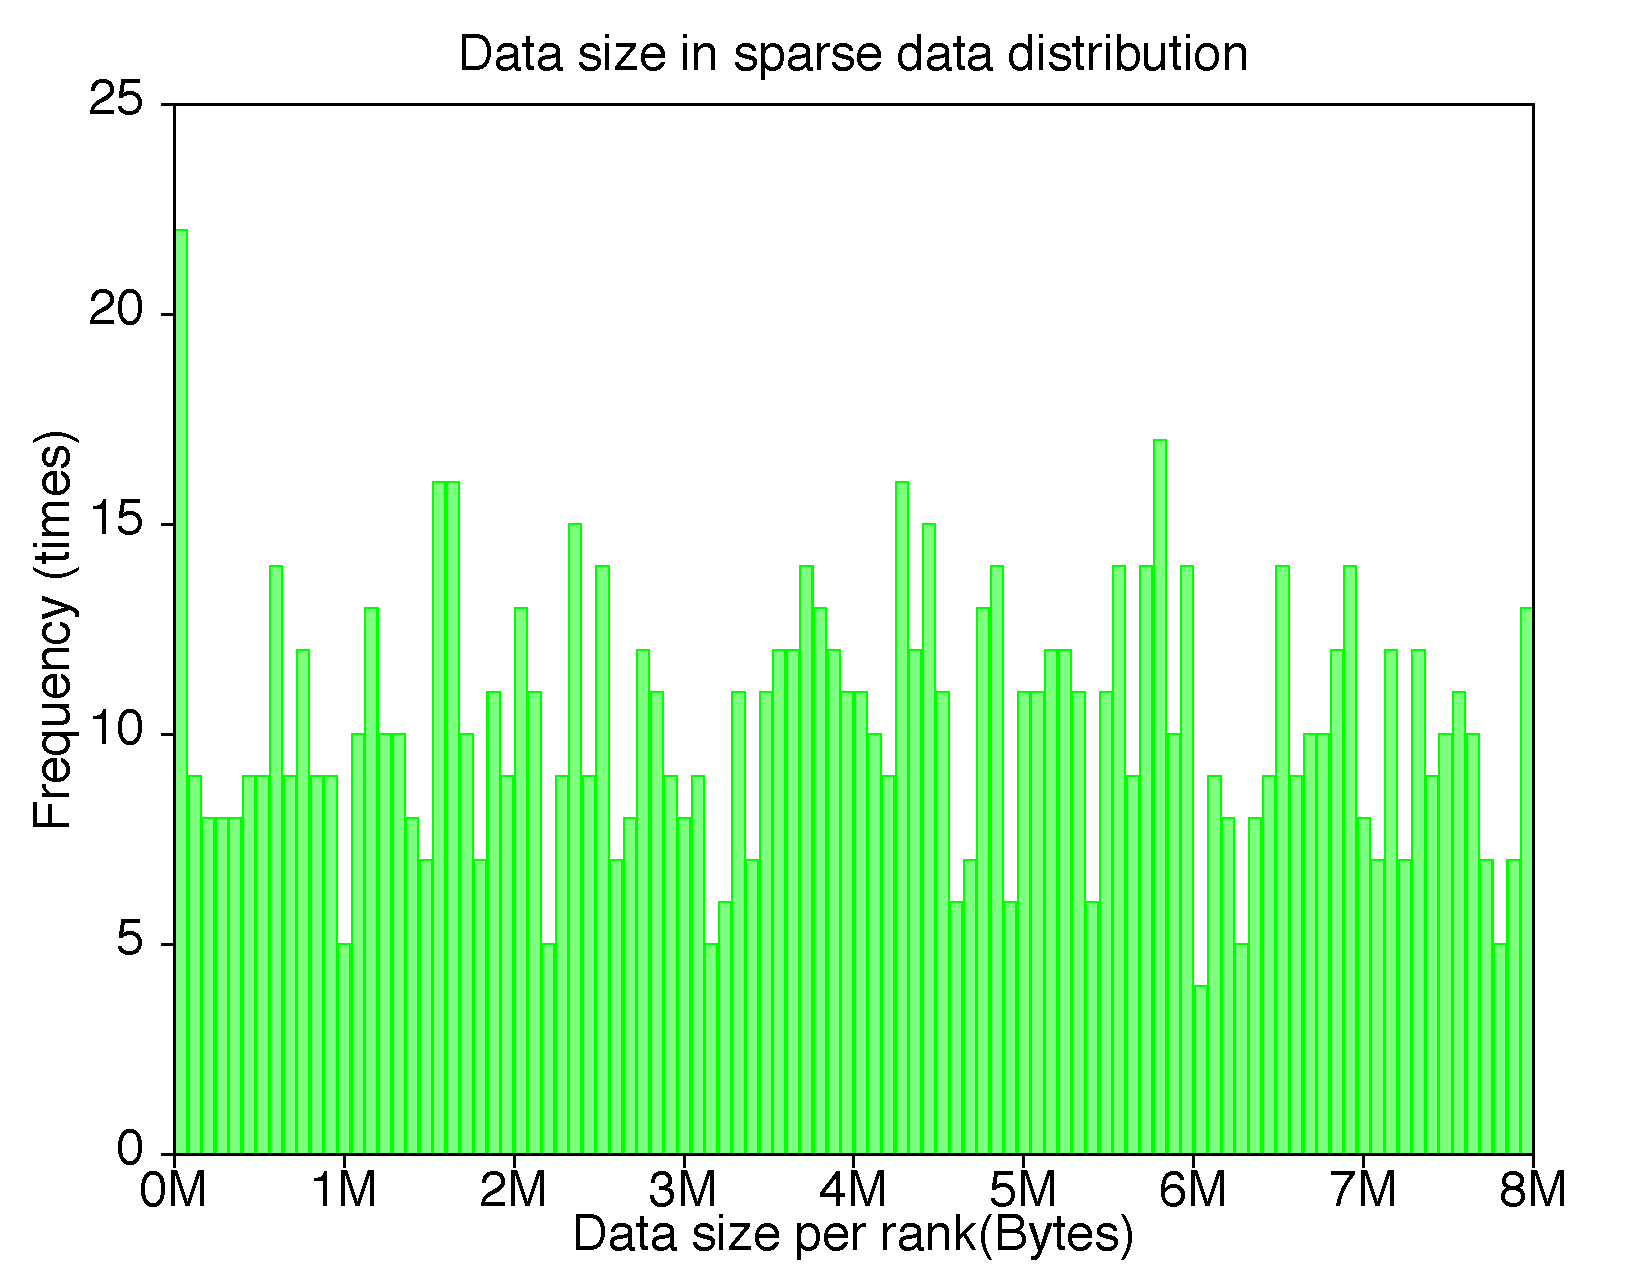
\includegraphics[scale=0.3]{figures/uniform.pdf}
\caption{Pattern 1: Histogram of data sizes for 1,024 processes using time(NULL) function with size from 0 to 8MB}
\label{fig:uniform}
\vspace{-0.1in}
\end{figure}

On the other hand, the data pattern 2 represents the case where data are sparse but not uniformly distributed. There are many nodes with almost no data while some nodes have large volume of data. This data pattern happens where we want to write out data from a region of contiguous MPI ranks while ignoring other regions.

\begin{figure}[!htb]
\vspace{-0.1in}
\centering
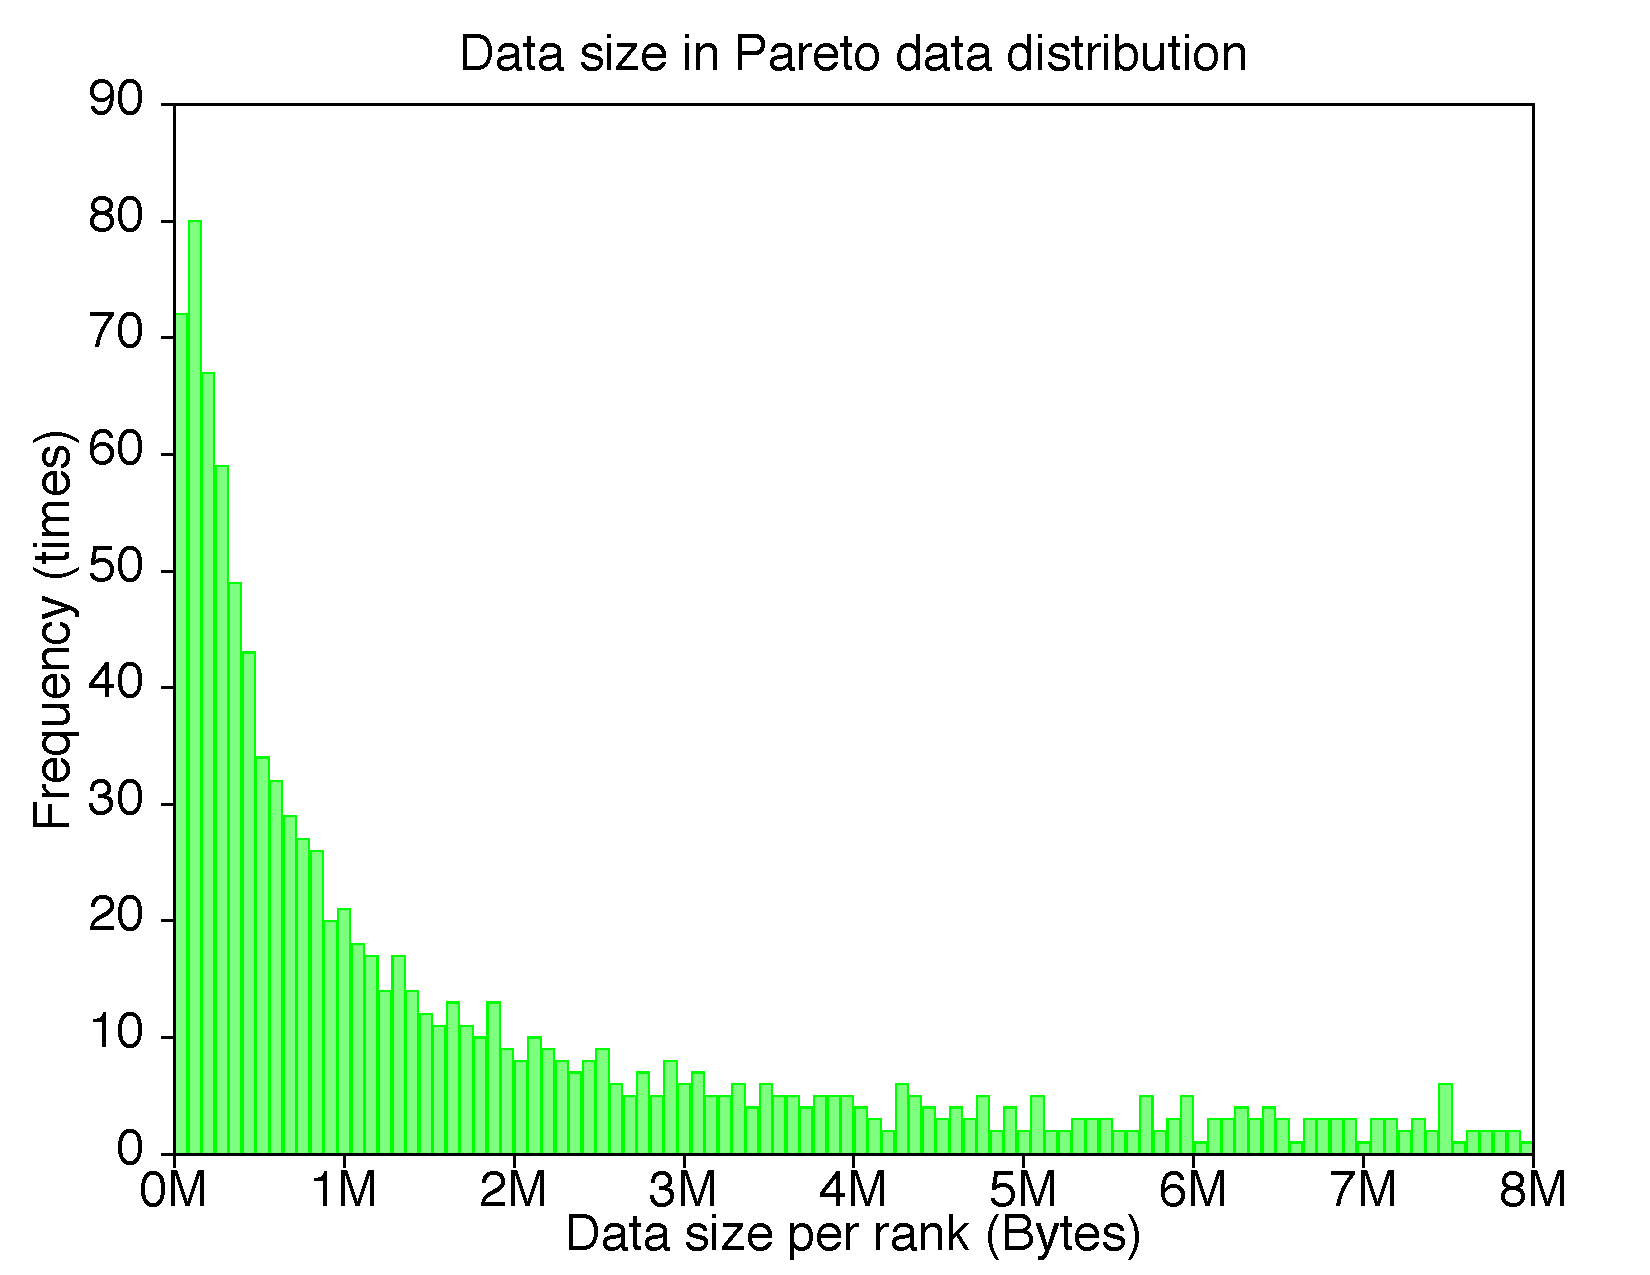
\includegraphics[scale=0.3]{figures/pareto.pdf}
\vspace{-0.1in}
\caption{Pattern 2: Histogram of data sizes of 1,024 processes using Pareto distribution function with size from 0B to 8MB}
\label{fig:pareto}
\vspace{-0.1in}
\end{figure}

On data pattern 1, we write roughly 8GB at 2,048 cores and 274GB of data at 131,072 cores. On data pattern 2, we write 3.4GB at 2,048 cores to 119GB of data at 131,072 cores. We compare the performance of performing aggregation for 2 data patterns using our approach and default MPI Collective I/O.

\begin{figure}[!htb]
\vspace{-0.1in}
\centering
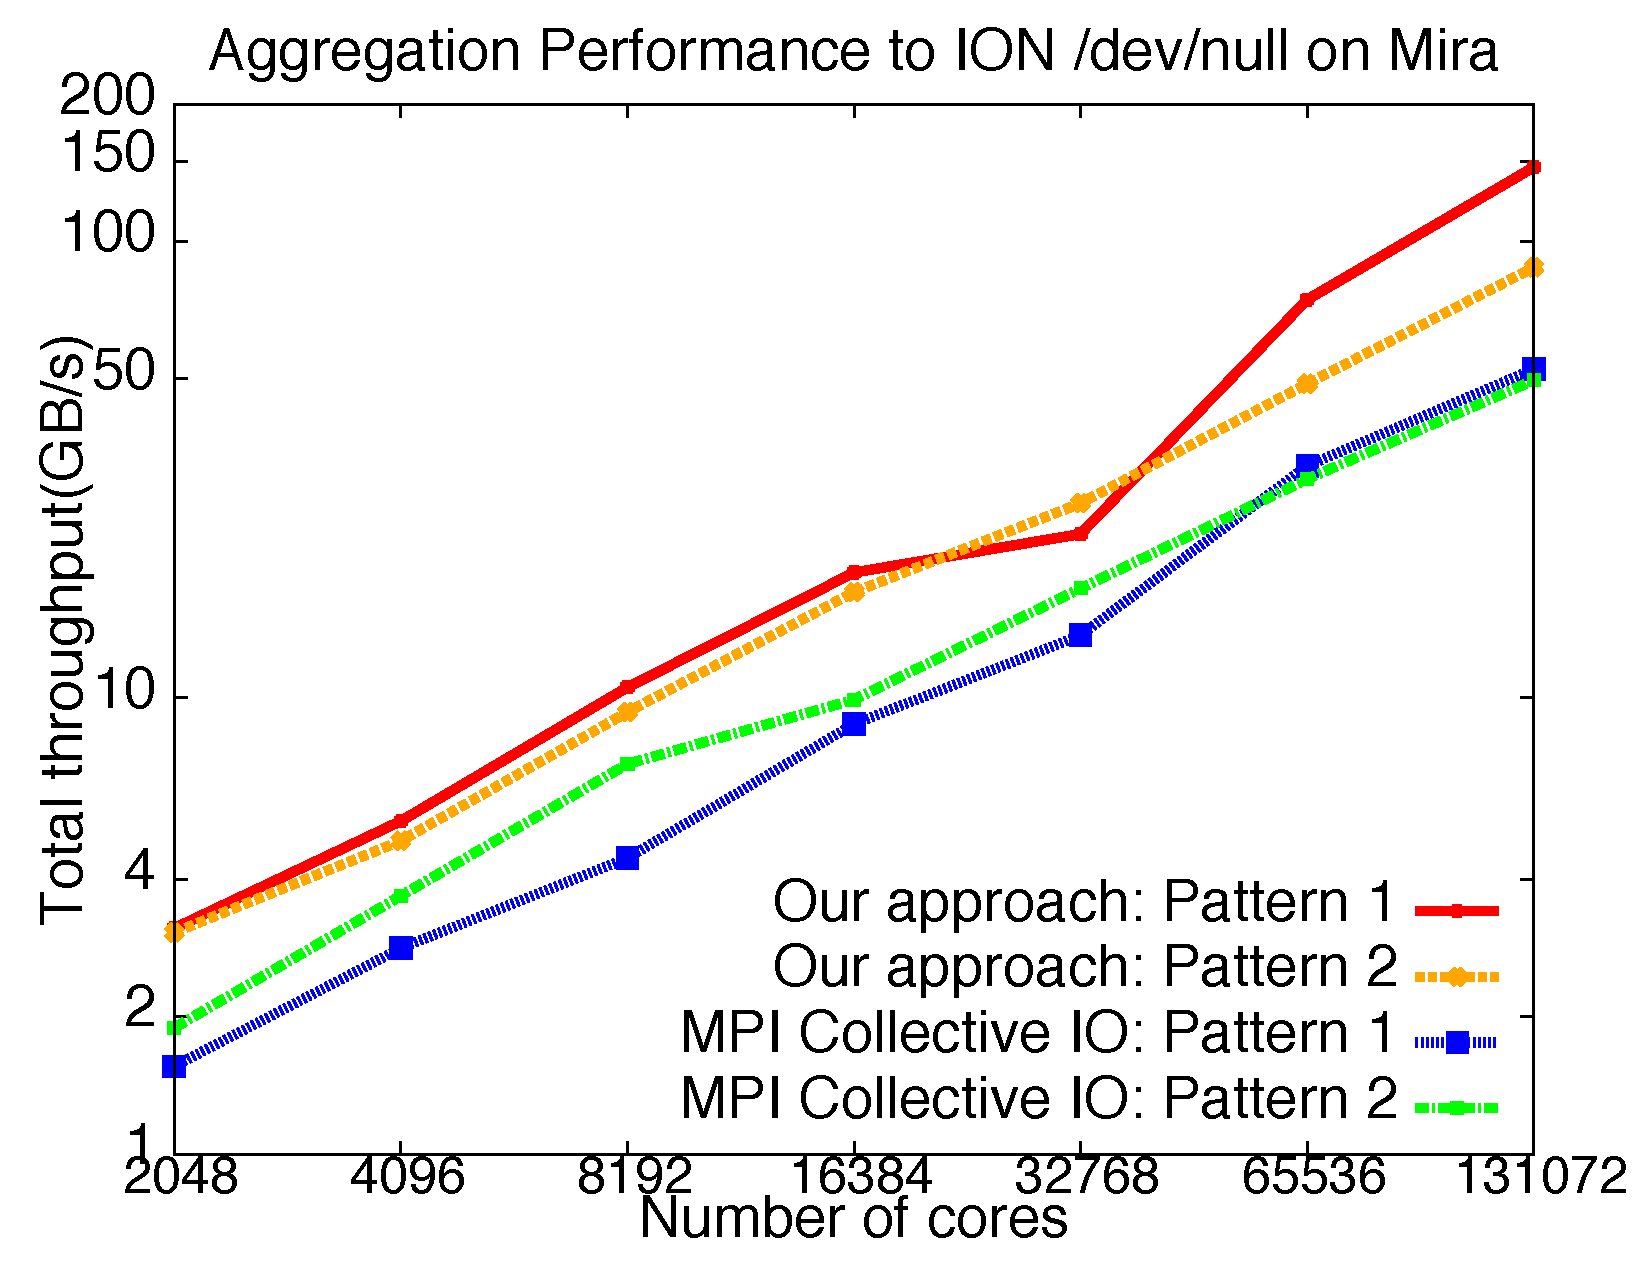
\includegraphics[scale=0.3]{figures/mira_agg.pdf}
\vspace{-0.2in}
\caption{Aggregation throughputs on Mira}
\vspace{-0.2in}
\label{fig:mira_agg}
\end{figure}

Figure \ref{fig:mira_agg} depicts the performance of our topology-aware multipath data movement approach in comparison to the default MPI-I/O for the two sparse data patterns as we scale from 2,048 cores to 131,072 cores on the Mira BG/Q system. On the data pattern 1 (uniformly distributed data), we observe  $2\times$ improvement at 2,048 cores. The performance increases as we scale and we achieve up to $3\times$ at 131,072 cores. On the data pattern 2 (pareto distributed data), we gain $1.5\times$ improvement at 2,048 cores and $2\times$ improvement at 131,072 cores. Thus, we observe that leveraging network interconnect topology and multipaths plays an important role at small scale and is critical at large scale. With the increased use of in-situ analysis for supercomputing,  sparse data patterns for I/O are becoming increasingly important and our approaches help provide more insights for improved performance.

\section{Application I/O benchmark}
\label{sec:app_benchmarks}
In this section, we demonstrate our solution on HACC I/O representing data movement between compute nodes and I/O nodes.

\subsection {HACC I/O}
HACC (Hardware/Hybrid Accelerated Cosmology Code) \cite{Habib:HACC} is a large-scale cosmology code suite that simulates the evolution of the universe through the first 13 billion years after the Big Bang. The simulation tracks the movement of trillions of particles as they collide and interact with each other, forming structure that transform into galaxies. During the runtime, HACC writes data periodically to storage system. The data can also be transferred from Mira to Tukey for data analysis and visualization. In both ways, data needs to go from compute nodes to I/O nodes first. In this benchmark, we use HACC I/O, an I/O benchmark written to evaluate performance of the I/O system for HACC, to show the data transfer performance from compute nodes to I/O nodes by writing to /dev/null. We compare the throughput of our mechanism to default MPI collective write on HACC I/O.
%\subsection{Staging}
%Presenting staging data from Mira to vis cluster Tukey. Analyze the results.

\subsection{Transferring data to I/O nodes}
In this experiments, we scale our experiments from 8,192 up to 131,072 compute cores to simulate the collision of $768^3$ to $2,816^3$ particles. We write only 10\% of the generated data with the amount of 2GB to 85GB of data. The data is written from processes with MPI ranks within the range [4*num\_processes/10, 5*num\_processes/10] with the num\_processes being the total number of MPI ranks in our application. We collect the bandwidth information and report the average. The results are shown in Figure \ref{fig:hacc_agg}

\begin{figure}[!htb]
\vspace{-0.1in}
\centering
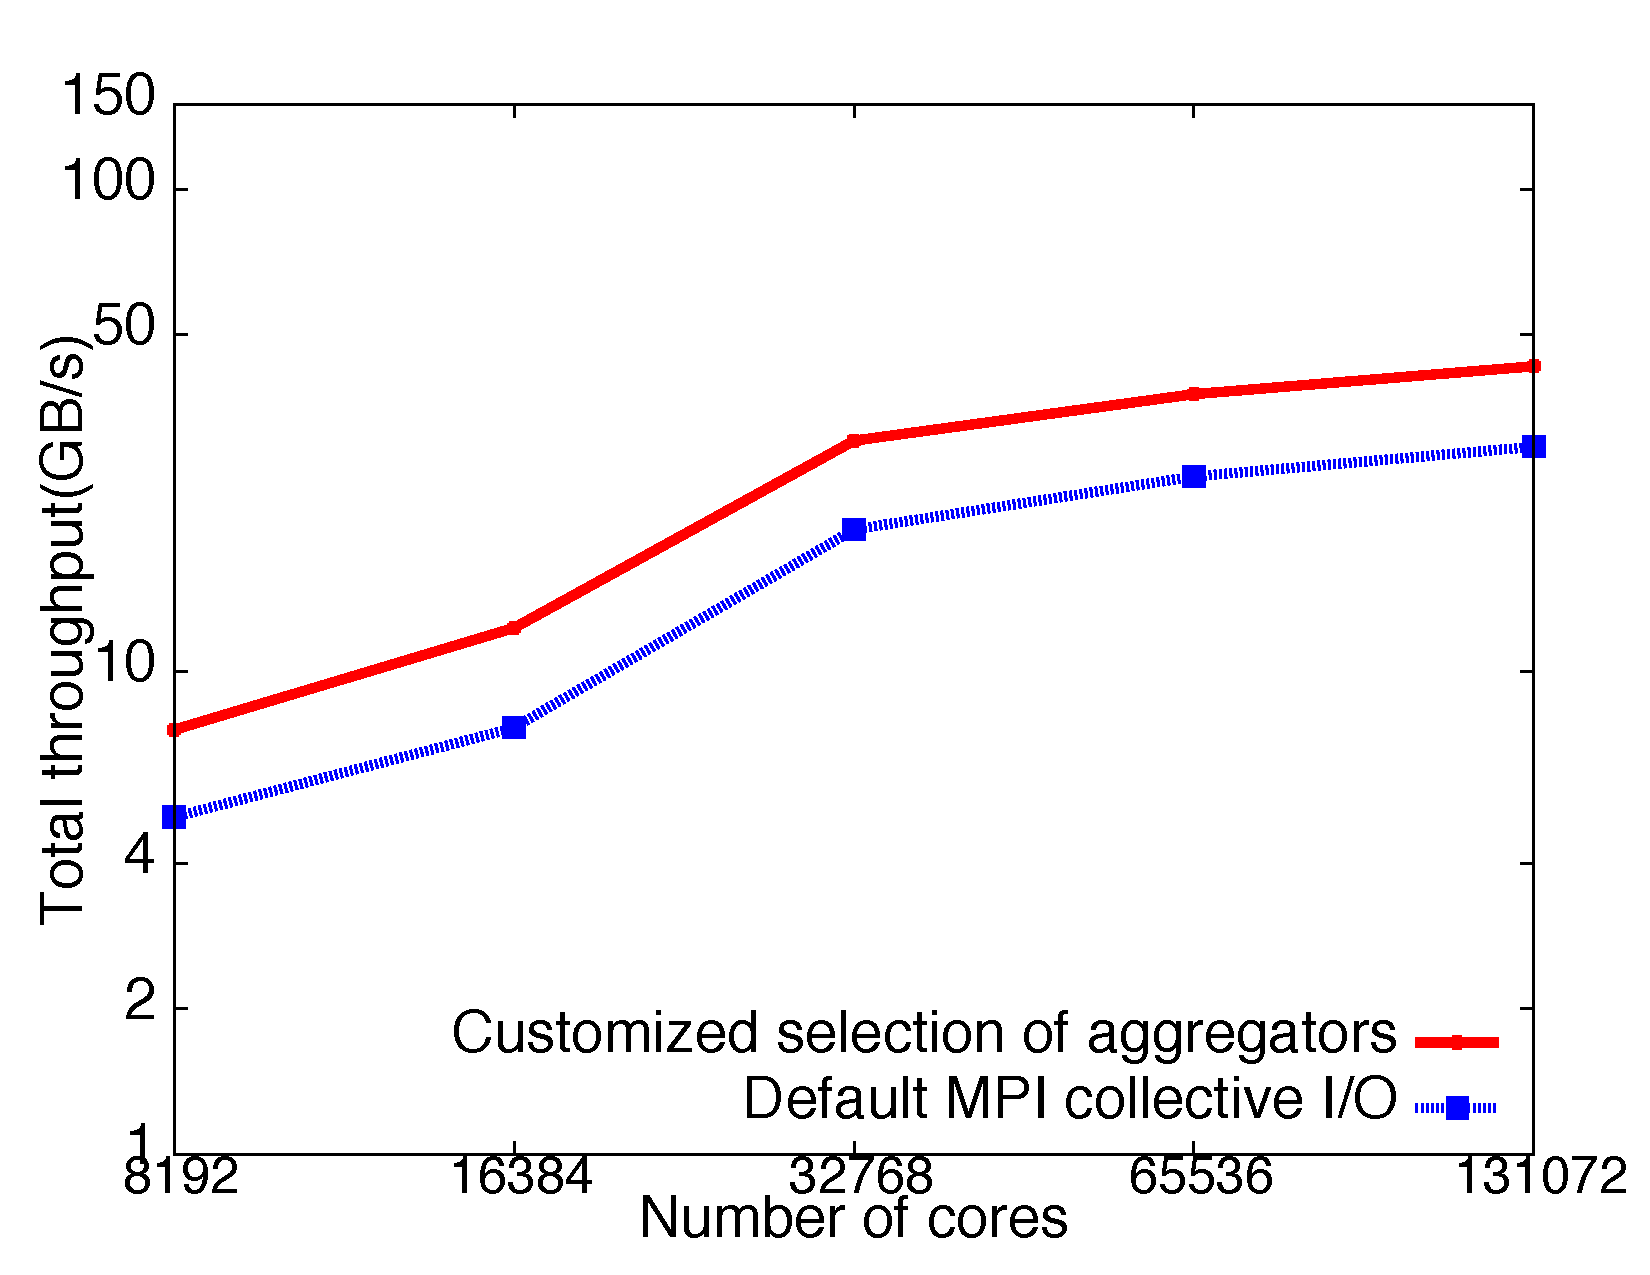
\includegraphics[scale=0.3]{figures/hacc_agg.pdf}
\vspace{-0.1in}
\caption{Write throughput of HACC application to I/O nodes /dev/null}
\vspace{-0.1in}
\label{fig:hacc_agg}
\end{figure}

The results show that in both cases, the number of I/O nodes employed is more than default I/O nodes. However, in our case, the position and location of aggregators are chosen dynamically and are distributed uniformly brought in better performance. Overall we can get up to 50\% throughput improvement. Thus, dynamic selection of number of and location of aggregators based on size of data and interconnect topology is of paramount importance for sparse data movement.

\subsection{Energy consumption comparison}
In these micro-benchmarks, we show that when using multi-path data movement for sparse data patterns, we not only increase bandwidth but also save energy consumption by the system.

\begin{figure}[!htb]
\vspace{-0.1in}
\centering
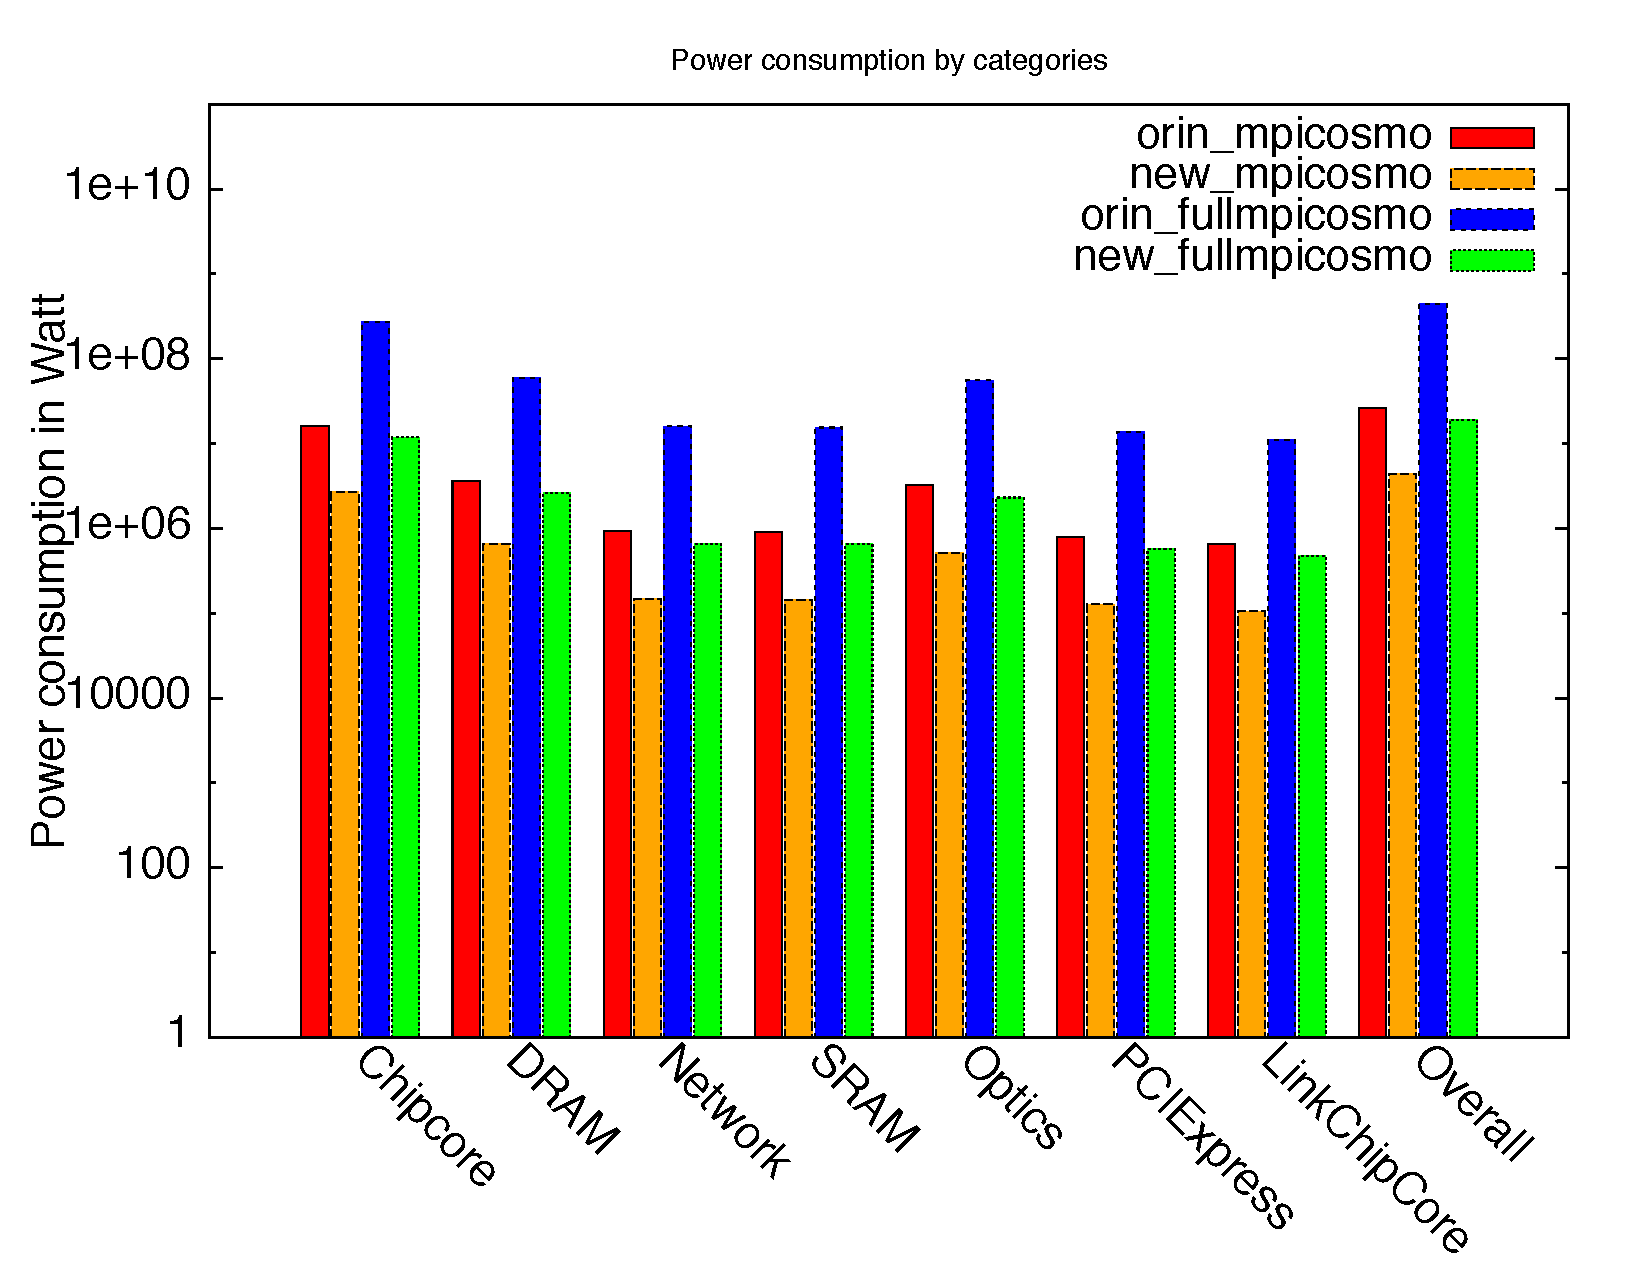
\includegraphics[scale=0.3]{figures/power_cat.pdf}
\vspace{-0.1in}
\caption{Energy consumption by category at a node}
\vspace{-0.1in}
\label{fig:hacc_agg}
\end{figure}

\begin{figure}[!htb]
\vspace{-0.1in}
\centering
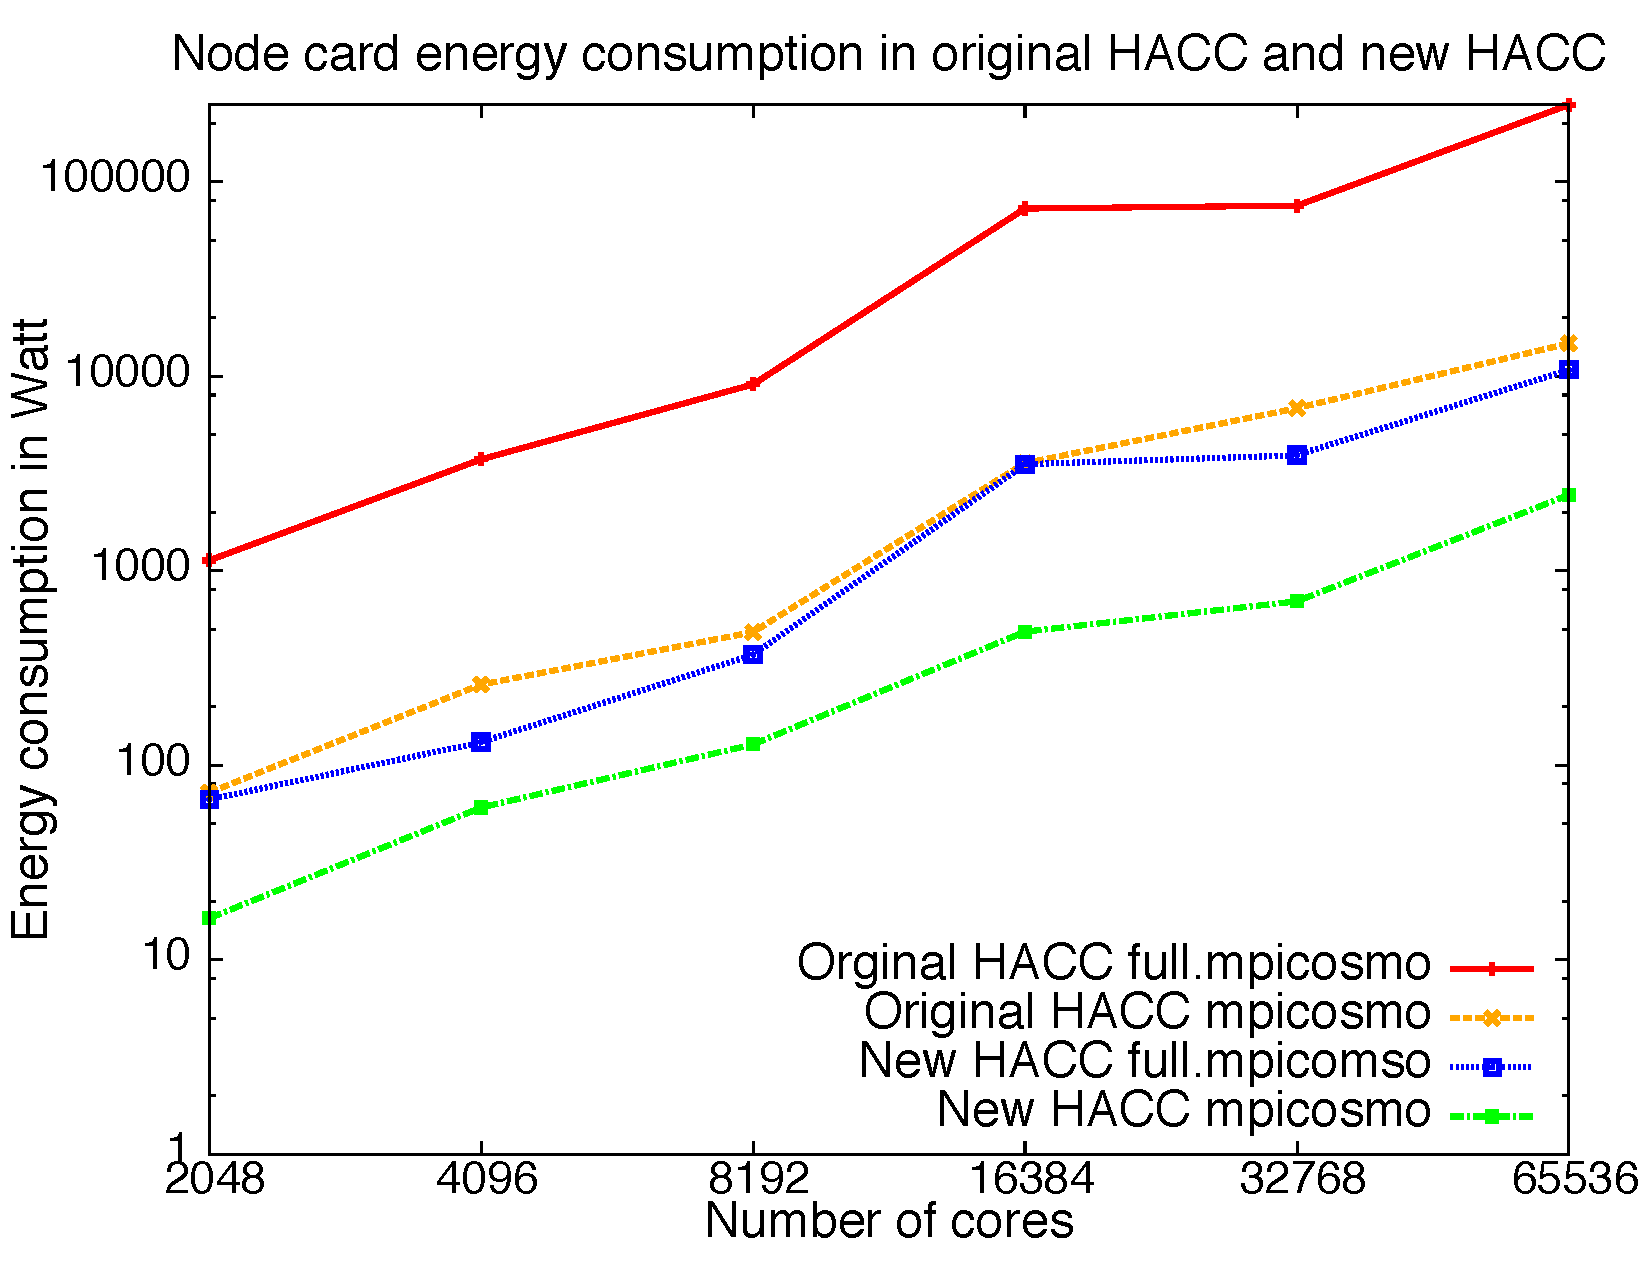
\includegraphics[scale=0.3]{figures/power_ncp.pdf}
\vspace{-0.1in}
\caption{Total energy consumption at scale}
\vspace{-0.1in}
\label{fig:hacc_agg}
\end{figure}


\section{Conclusion}
\label{sec:conclusion}
%In this paper 
We proposed two approaches for balancing load on the Blue Gene/Q supercomputer using multiple paths for data movement. We realized our approaches in OPTIQ framework and demonstrated the efficacy of our work through a set of benchmarks. Overall, we improved throughput by 43\%--67\% on average for three different communication patterns in 91 experiments on up to 4096 nodes. %Performance, however, can be improved up to 4X. %what does this mean? 
Our work shows that to improve data movement performance we need to take advantage of both application's data movement patterns and system routing algorithms. In general, our Optimization approach outperforms heuristic and MPI\_Alltoallv due to better load-balanced multiple paths for data movement. In future, we plan to study these approaches on the Cray XE6 supercomputer and test them with real applications.


\section*{Acknowledgments}

This research used resources of the Argonne Leadership Computing Facility (ALCF) at Argonne National Laboratory, and is supported by the Office of Science of the U.S. Department of Energy under contract DE-AC02-06CH11357. We thank the ALCF team for discussions and help related to this paper.

%% The Appendices part is started with the command \appendix;
%% appendix sections are then done as normal sections
%% \appendix

%% \section{}
%% \label{}

\section*{References}

%% If you have bibdatabase file and want bibtex to generate the
%% bibitems, please use
%%
\bibliographystyle{elsarticle-num} 
\bibliography{sigproc}

%% else use the following coding to input the bibitems directly in the
%% TeX file.

%\begin{thebibliography}{00}

%% \bibitem{label}
%% Text of bibliographic item

%% \bibitem{}

%\end{thebibliography}
\end{document}
\endinput
%%
%% End of file `elsarticle-template-num.tex'.
